\section{DASH}

\subsection{Overview}

Dynamic Adaptive Streaming over HTTP (DASH) is a protocol, defined in
ISO/IEC 23009-1~\cite{iso-dash-2014}, that facilitates 
streaming of multimedia over the internet in varying network conditions.
The goal of DASH and other segment-based streaming service structures is to improve the user
experience~\cite{Google I/O 2013} while streaming media content by splitting the media file in question
into smaller parts and letting the streaming client choose between several
different versions of the same file depending on preferred quality and network
conditions. In effect, it allows streaming clients the ability to aggressively
limit stalling in video playback at the cost of perceived video/audio quality
while simultaneously saving the service provider a significant amount of
network traffic~\cite[p. 412]{dashing-youtube}~\cite{Google I/O 2013}.

The core of DASH is the Media Presentation Description (MPD), sometimes
referred to as the DASH manifest. The MPD contains all the information
needed to display the media. When a user wants to access a streamed
media (for instance a video) the streaming client (or website frontend)
makes a request to get the MPD for the requested media. The client then
parses the MPD and measures available network and buffer resources,
before the streaming is commenced at the best feasible quality. Many clients %TODO: references?
seem to prefer starting the stream at the lowest available quality, and
slowly ramp the quality up if no network problems occur. The
client continues to monitor the available resources during playback, adapting
quality dynamically if conditions should change.

With this approach all decisions about download speed are left to the client
alone.
The server simply presents the entirety of the media information in the MPD,
allowing the client to make its own informed choices. The client may choose
to focus on continuous playback, for instance by downloading lower quality
segments during heavy network congestion or local processor load, or it may
force playback of a set quality no matter the conditions under which it
operates. The behavioral pattern for most media streaming clients, among
others YouTube's own media player, seems to be to value continuous playback
over intermittent delays in high quality playback~\cite{Google I/O 2013}, unless the user should want
to force a specific quality setting thus overriding default behavior.

The developed tool only downloads the media files as specified by the
user, and does not care about available resources or the user experience.
The DASH manifest is still parsed, and all relevant data is stored in the
database to provide an overview of the available medias, qualities,
and their respective properties. Although we are not using DASH to
accomplish better user experience, the MPD is still very useful as a
single point to get information about a streamed media.

\subsection{Media Presentation Description}

\begin{figure}
    \centering
    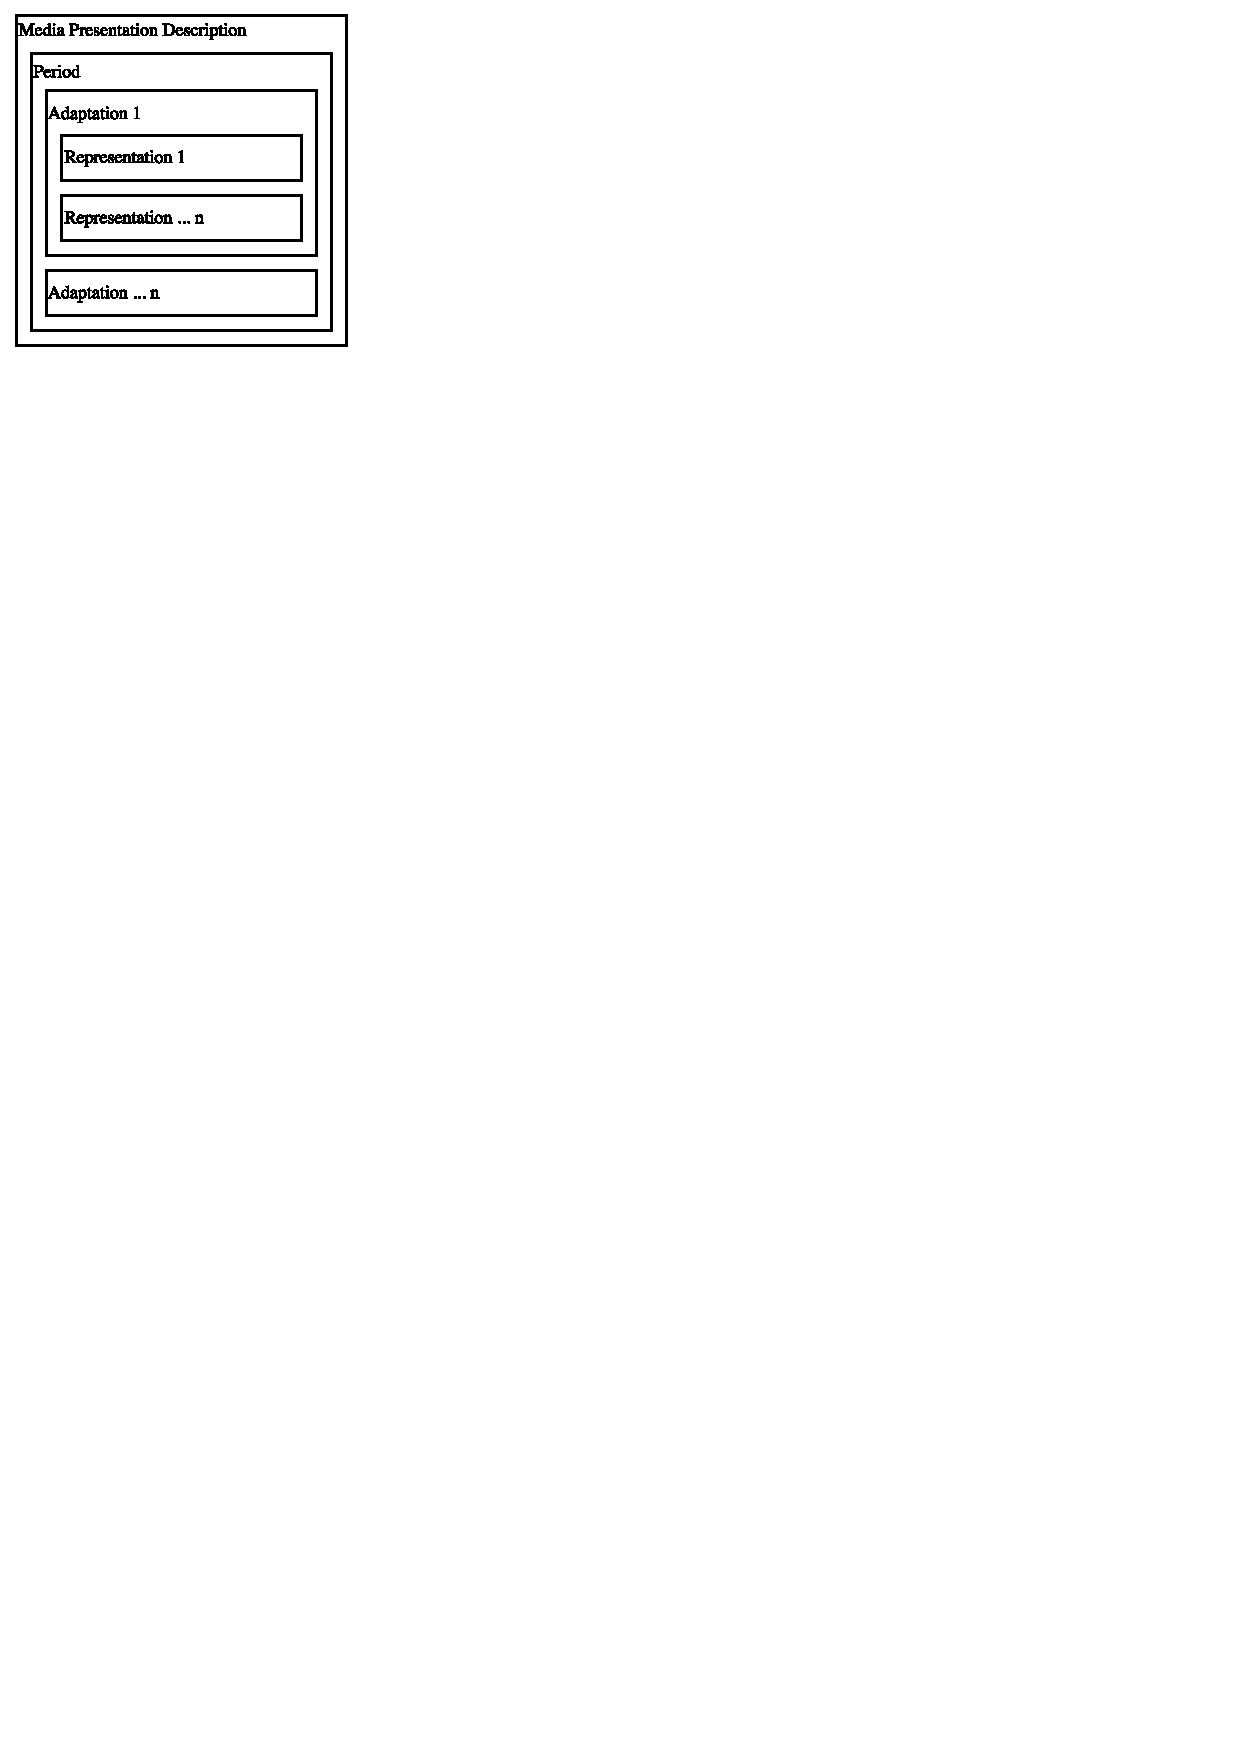
\includegraphics[width=0.4\textwidth]{figures/dash-mpd-diagram}
    \caption{Diagram of the YouTube Media Presentation Description.}
    \label{fig:dash-mpd-diagram}
\end{figure}

~\cref{fig:dash-mpd-diagram} depicts the basic outline of a Media Presentation
Description. The uppermost layer of the YouTube MPD contains duration of the
media as well as information about the format. Each MPD contains a set of
adaptations, each describing a media type. An arbitrary YouTube video might have
the following adaptations: Audio/mp4, audio/webm, video/mp4, video/webm. There
are also different adaptations for 3D videos, live media streams, etc. Each
adaptation (media type) might have multiple representations each designating a
different media quality.

Note that this differs from what one might consider the \textit{standard ISO
DASH}\footnote{The DASH standard is incredibly loose in order to allow different
implementations and the freedom to make changes that benefit the specific media
host the most, thus there is not really a \textit{standard} DASH implementation.}
implementation. The standard facilitates using periods to
describe discrete segments within the media, with each period containing links
to separate files containing separate quality versions of that same period.
YouTube works differently: There is only one period, with several adaptations
describing different media types, each with several representations describing
different qualities of media. YouTube MPD representations contain a single file\footnote{Or more specifically, a single URI}
containing the entire video in the quality specified in the representation.
The media player client does not have to do anything more advanced than simply
request this file in order to play the designated media. If it is to utilize
DASH, however, it needs to calculate which chunks of which file it needs to
fetch in order to assure smooth playback.

\subsection{Representation details}

\begin{figure}
    \centering
    \begin{lstlisting}[
        basicstyle = \footnotesize\ttfamily
    ]
    {
        "@id": "137",
        "@codecs": "avc1.640028",
        "@width": "1920",
        "@height": "1080",
        "@startWithSAP": "1",
        "@maxPlayoutRate": "1",
        "@bandwidth": "4133205",
        "@frameRate": "24",
        "BaseURL": {
            "@yt:contentLength": "148765820",
            "#text": [OMITTED - URI goes here]
        },
        "SegmentBase": {
            "@indexRange": "711-1942",
            "@indexRangeExact": "true",
            "Initialization": {
                "@range": "0-710"
            }
        }
    }
    \end{lstlisting}
    \caption{Example of an mp4 1080p (\textit{full HD}) representation}
    \label{fig:dash-1080p-representation}
\end{figure}

\subsubsection{\texttt{@id}}
Specifies a unique (within the Period) identifier for this Representation, used
for easy lookup and the
potential for (reckless!) hard-coding of identifiers instead of checking for
video parameters as strings.
Each id is linked with a specific type of video. In the case of
YouTube's version of MPDs, $137$ is defined to always be a 1920x1080 mp4 video, for
example~\cite[line 303]{youtube-dl:youtube.py}\footnote{The retrieval of MPD's
does not seem to be officially supported in the YouTube API v3, thus there are
no truly reliable sources. The reference is to a popular YouTube downloader tool
that seems to have figured out how the MPD is laid out as of 2015-11-01}

\subsubsection{\texttt{@codecs}}
Specifies the codecs present with this
Representation. The field should also include the profile and level
information where applicable. For this video,~\cref{fig:dash-1080p-representation}, the codec specifies a
H.264/AVC video, High Profile, Level 40~\cite[p. 12]{rfc6381}.

\subsubsection{\texttt{@width} and \texttt{@height}}
Specifies the resolution of the video in pixels.

\subsubsection{\texttt{@startWithSAP}}
The SAP, or Stream Access Point, describes a position in a Representation
enabling playback of a media stream to be started using only the information
contained in Representation data starting form that position
onwards~\cite[p. 11]{iso-dash-2014}. The usage of this type of parameter
is not specified exactly in the standard, but its general use is described.
In other words, using this attribute and only the attributes in the
current Representation, the player must be able to play the media segment
described by the current Period.

\subsubsection{\texttt{@maxPlayoutRate}}
Specifies the maximum playout rate as a multiple of the
regular playout rate. In ~\cref{fig:dash-1080p-representation} it is set to 1: It is not supported.

\subsubsection{\texttt{@bandwidth}}
A little more complicated than the other fields.
If a Representation is continuously delivered at this bitrate in a
constant bitrate channel of \texttt{@bandwidth} bits per second starting at
SAP 1, a client
can be assured of having enough data for continuous playback providing
playout begins after \texttt{@minBufferTime} * \texttt{@bandwidth} bits have been
received. In short: If the client is able to maintain a download rate
consistently equal to or greater than \texttt{@bandwidth} during the entire
playback, the user will never experience stalling.

\subsubsection{Other}
Not all identifiers are specified in the ISO DASH standard. YouTube
provides some of its own, and these are prefixed with \textit{yt:}.
The \texttt{@yt:contentLength} field, for example, specifies the size of the
Representation in bytes.

When switching from Presentation $X$ to Presentation $Y$ at segment $n$, the
\texttt{@baseURL/\#text} (URI describing the media resource of Presentation $Y$)
is used in conjunction with \texttt{@bandwidth} of Presentation $Y$ to
calculate the chunk offset of segment $n+1$ into the media file.

